\chapter{Il sistema Ball and Plate}
\label{chapter:ballandplate}

Il termine \textbf{Ball and Plate} si riferisce ad un sistema che presenta un piano con quattro assi di libertà sopra il quale è presente una sfera. Tramite un controllo opportuno è possibile cambiare l'inclinazione del piano affinché la sfera raggiunga una posizione desiderata, o addirittura affinché segua delle traiettorie prestabilite.

Il sistema Ball and Plate è un'estensione a due dimensioni del più semplice sistema chiamato \textbf{Ball and Beam}.

\section{Ball and Beam}

In questa sezione viene brevemente espresso il modello matematico di un sistema Ball and Beam\cite{ballandbeam}.

\bigskip

\begin{figure}[ht]

	\centering
	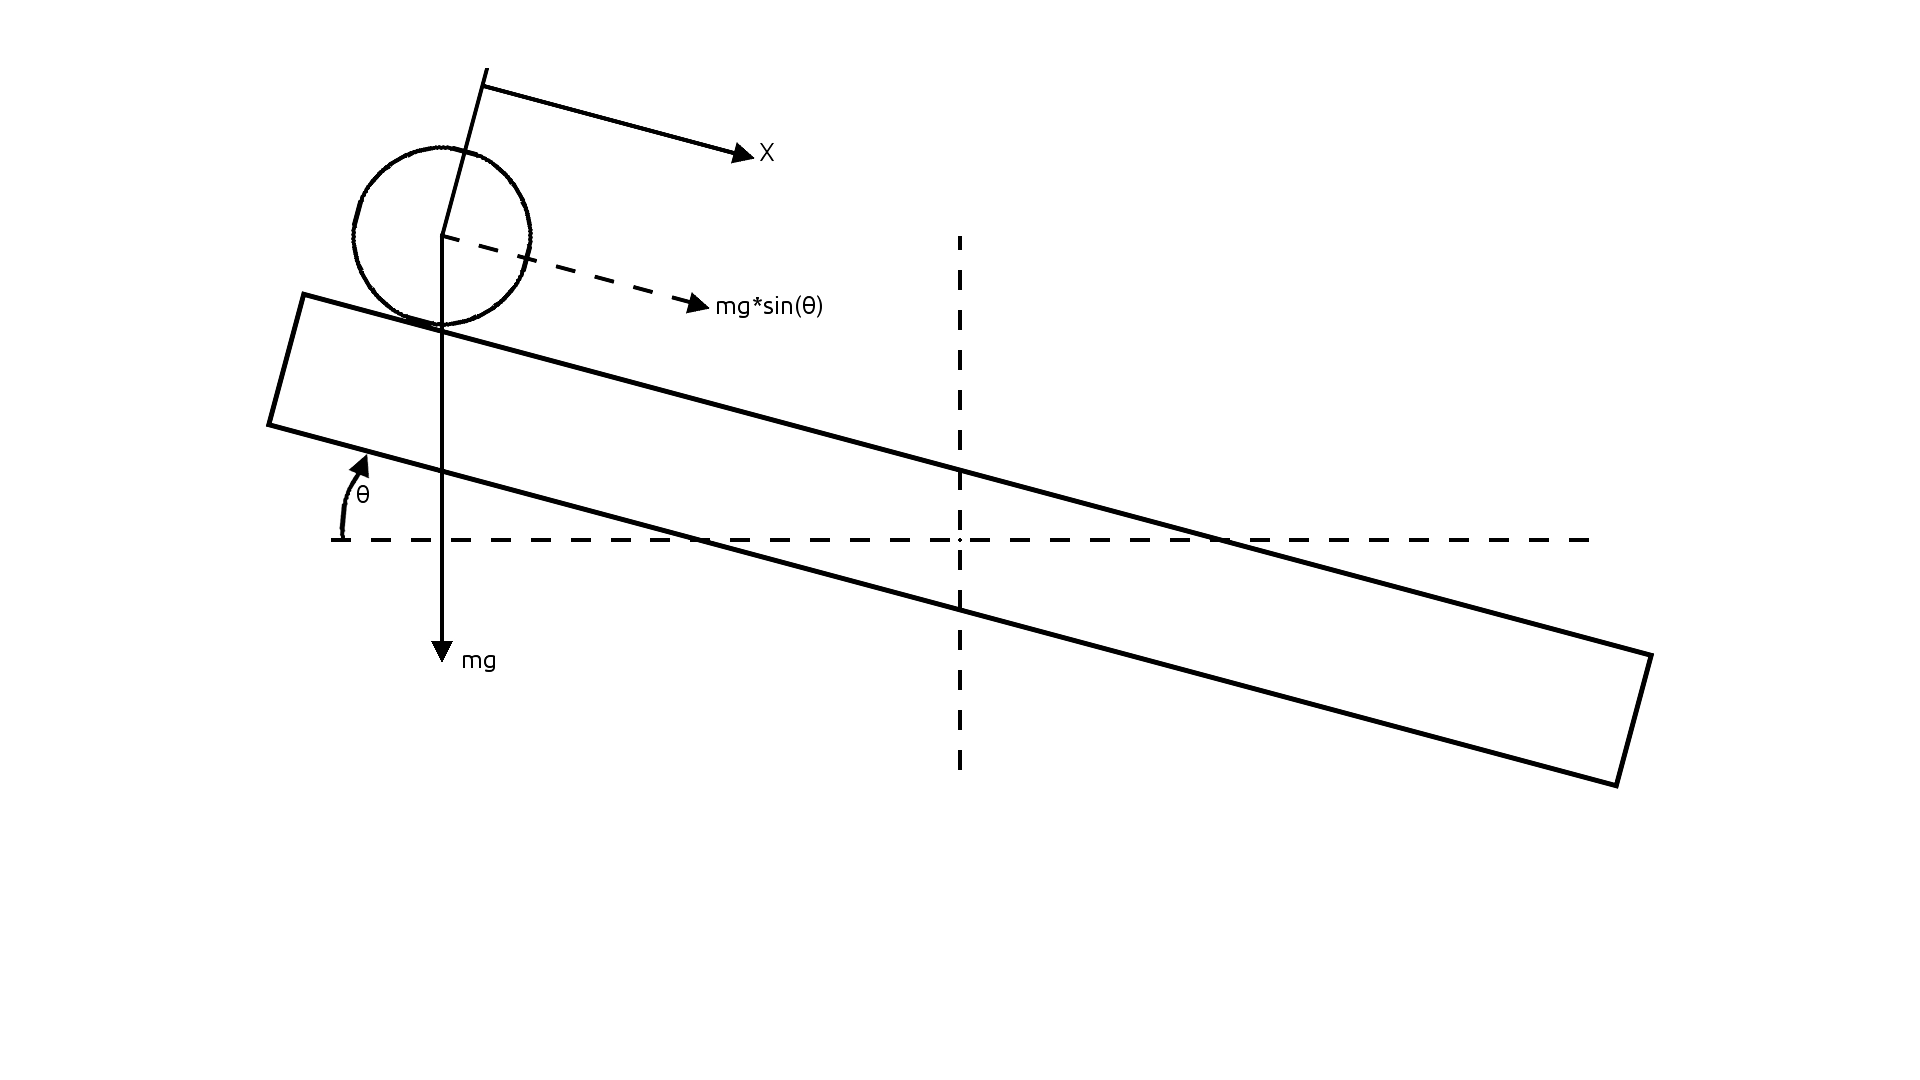
\includegraphics[width=\textwidth]{ballandbeam}
	\caption{Ball and Beam, modello fisico}
	\label{fig:ballandbeam}
\end{figure}

La forza applicata sulla sfera è causata dalla componente della gravitazionale che agisce in maniera parallela al'asse (\textit{Beam}). Come è possibile vedere in figura \ref{fig:ballandbeam}, questa forza vale $mg$sin$(\theta)$. Nonostante in realtà la sfera acceleri lungo l'asse tramite rotazione, possiamo semplificare il modello e assumere che scorra sopra di esso senza alcuna componente d'attrito. 

Il modello (semplificato) del sistema ball and beam è perciò il seguente:

\begin{equation}
	\centering
	mgsin(\theta) = m\ddot{x}
	\label{equation:firstmodel}
\end{equation}

Dove $m$ è la massa della sfera, $g$ è la costante gravitazionale, $\theta$ è l'angolo dell'asse e $x$ è la posizione della sfera lungo l'asse.

Per angoli piccoli è possibile approssimare sin$(\theta)$ con $\theta$, per cui il modello dell'equazione \ref{equation:firstmodel} diventa:

\begin{equation}
	\centering
	\ddot{x} = g\theta
	\label{equation:secondmodel}
\end{equation}

Questo modello mostra che l'accelerazione della sfera è proporzionale alla forza di gravità e all'angolo di inclinazione dell'asse. L'angolo d'incidenza dell'asse $\theta$ è proporzionale alla tensione $u$ impartita al motore responsabile di controllarne l'inclinazione, e la posizione della sfera viene letta da un sensore di posizione $y$. Rimpiazzando, all'interno dell'equazione \ref{equation:secondmodel}, $\theta$ con la tensione di controllo $u$, la posizione della sfera con l'output del sensore $y$ e unendo la costante gravitazionale con quelle del sensore e dell'attuatore si ottiene una singola costante $b$.

\begin{equation}
\centering
\ddot{y} = bu
\label{equation:finalmodel}
\end{equation}

\newpage
La funzione di trasferimento ottenuta dall'equazione \ref{equation:finalmodel} è l'equazione \ref{equation:babtf}:

\begin{equation}
\centering
x(s) = \frac{b}{s^{2}}u(s)
\label{equation:babtf}
\end{equation}

Posto che lo stato del sistema è definito dalla posizione della sfera $x_{1}$ e dalla sua velocità $x_{2}$, allora la rappresentazione in spazio di stato è l'equazione \ref{equation:babss}

\begin{align}
	\centering
	\begin{bmatrix}
		\dot{x}_{1} \\ \dot{x}_{2}
	\end{bmatrix}
	&= 
	\begin{bmatrix}
		0 & 1 \\ 0 & 0
	\end{bmatrix}
	\begin{bmatrix}
		x_{1} \\ x_{2}
	\end{bmatrix}
	+
	\begin{bmatrix}
		0 \\ b
	\end{bmatrix}u \nonumber
	\\
	y &=
	\begin{bmatrix}
		1 & 0
	\end{bmatrix}
	\begin{bmatrix}
		x_{1} \\ x_{2}
	\end{bmatrix}
	\label{equation:babss}
\end{align}

Nonostante questo sia il modello ideale (lineare) di un sistema ball and beam, un sistema reale (non lineare) presenta delle componenti aggiuntive quali
\begin{itemize}[noitemsep]
	\item Componente d'attrito
	\item Rumore del sensore di posizione
	\item Tempo di attuazione del servomotore
\end{itemize}

Ciononostante, data la sua semplicità, questa tipologia di sistema può essere facilmente controllata utilizzando un controllo di tipo Proporzionale-Derivativo (\textit{PD}). Ulteriori dettagli sulle tipologie di controllo sono presenti nel capitolo \ref{chapter:controllo}.

\section{Ball and Plate}

In questa sezione viene definito il modello matematico di un sistema Ball and Plate.

Nel definire il modello vengono fatte le seguenti ipotesi:
\begin{itemize}[noitemsep]
	\item La sfera è simmetrica ed omogenea
	\item Il contatto tra la sfera e il piano non viene mai perso
	\item La sfera non ha moto di solo strisciamento sul piano
	\item Gli attriti vengono trascurati
\end{itemize}

\bigskip

\begin{figure}[ht]
	\centering
	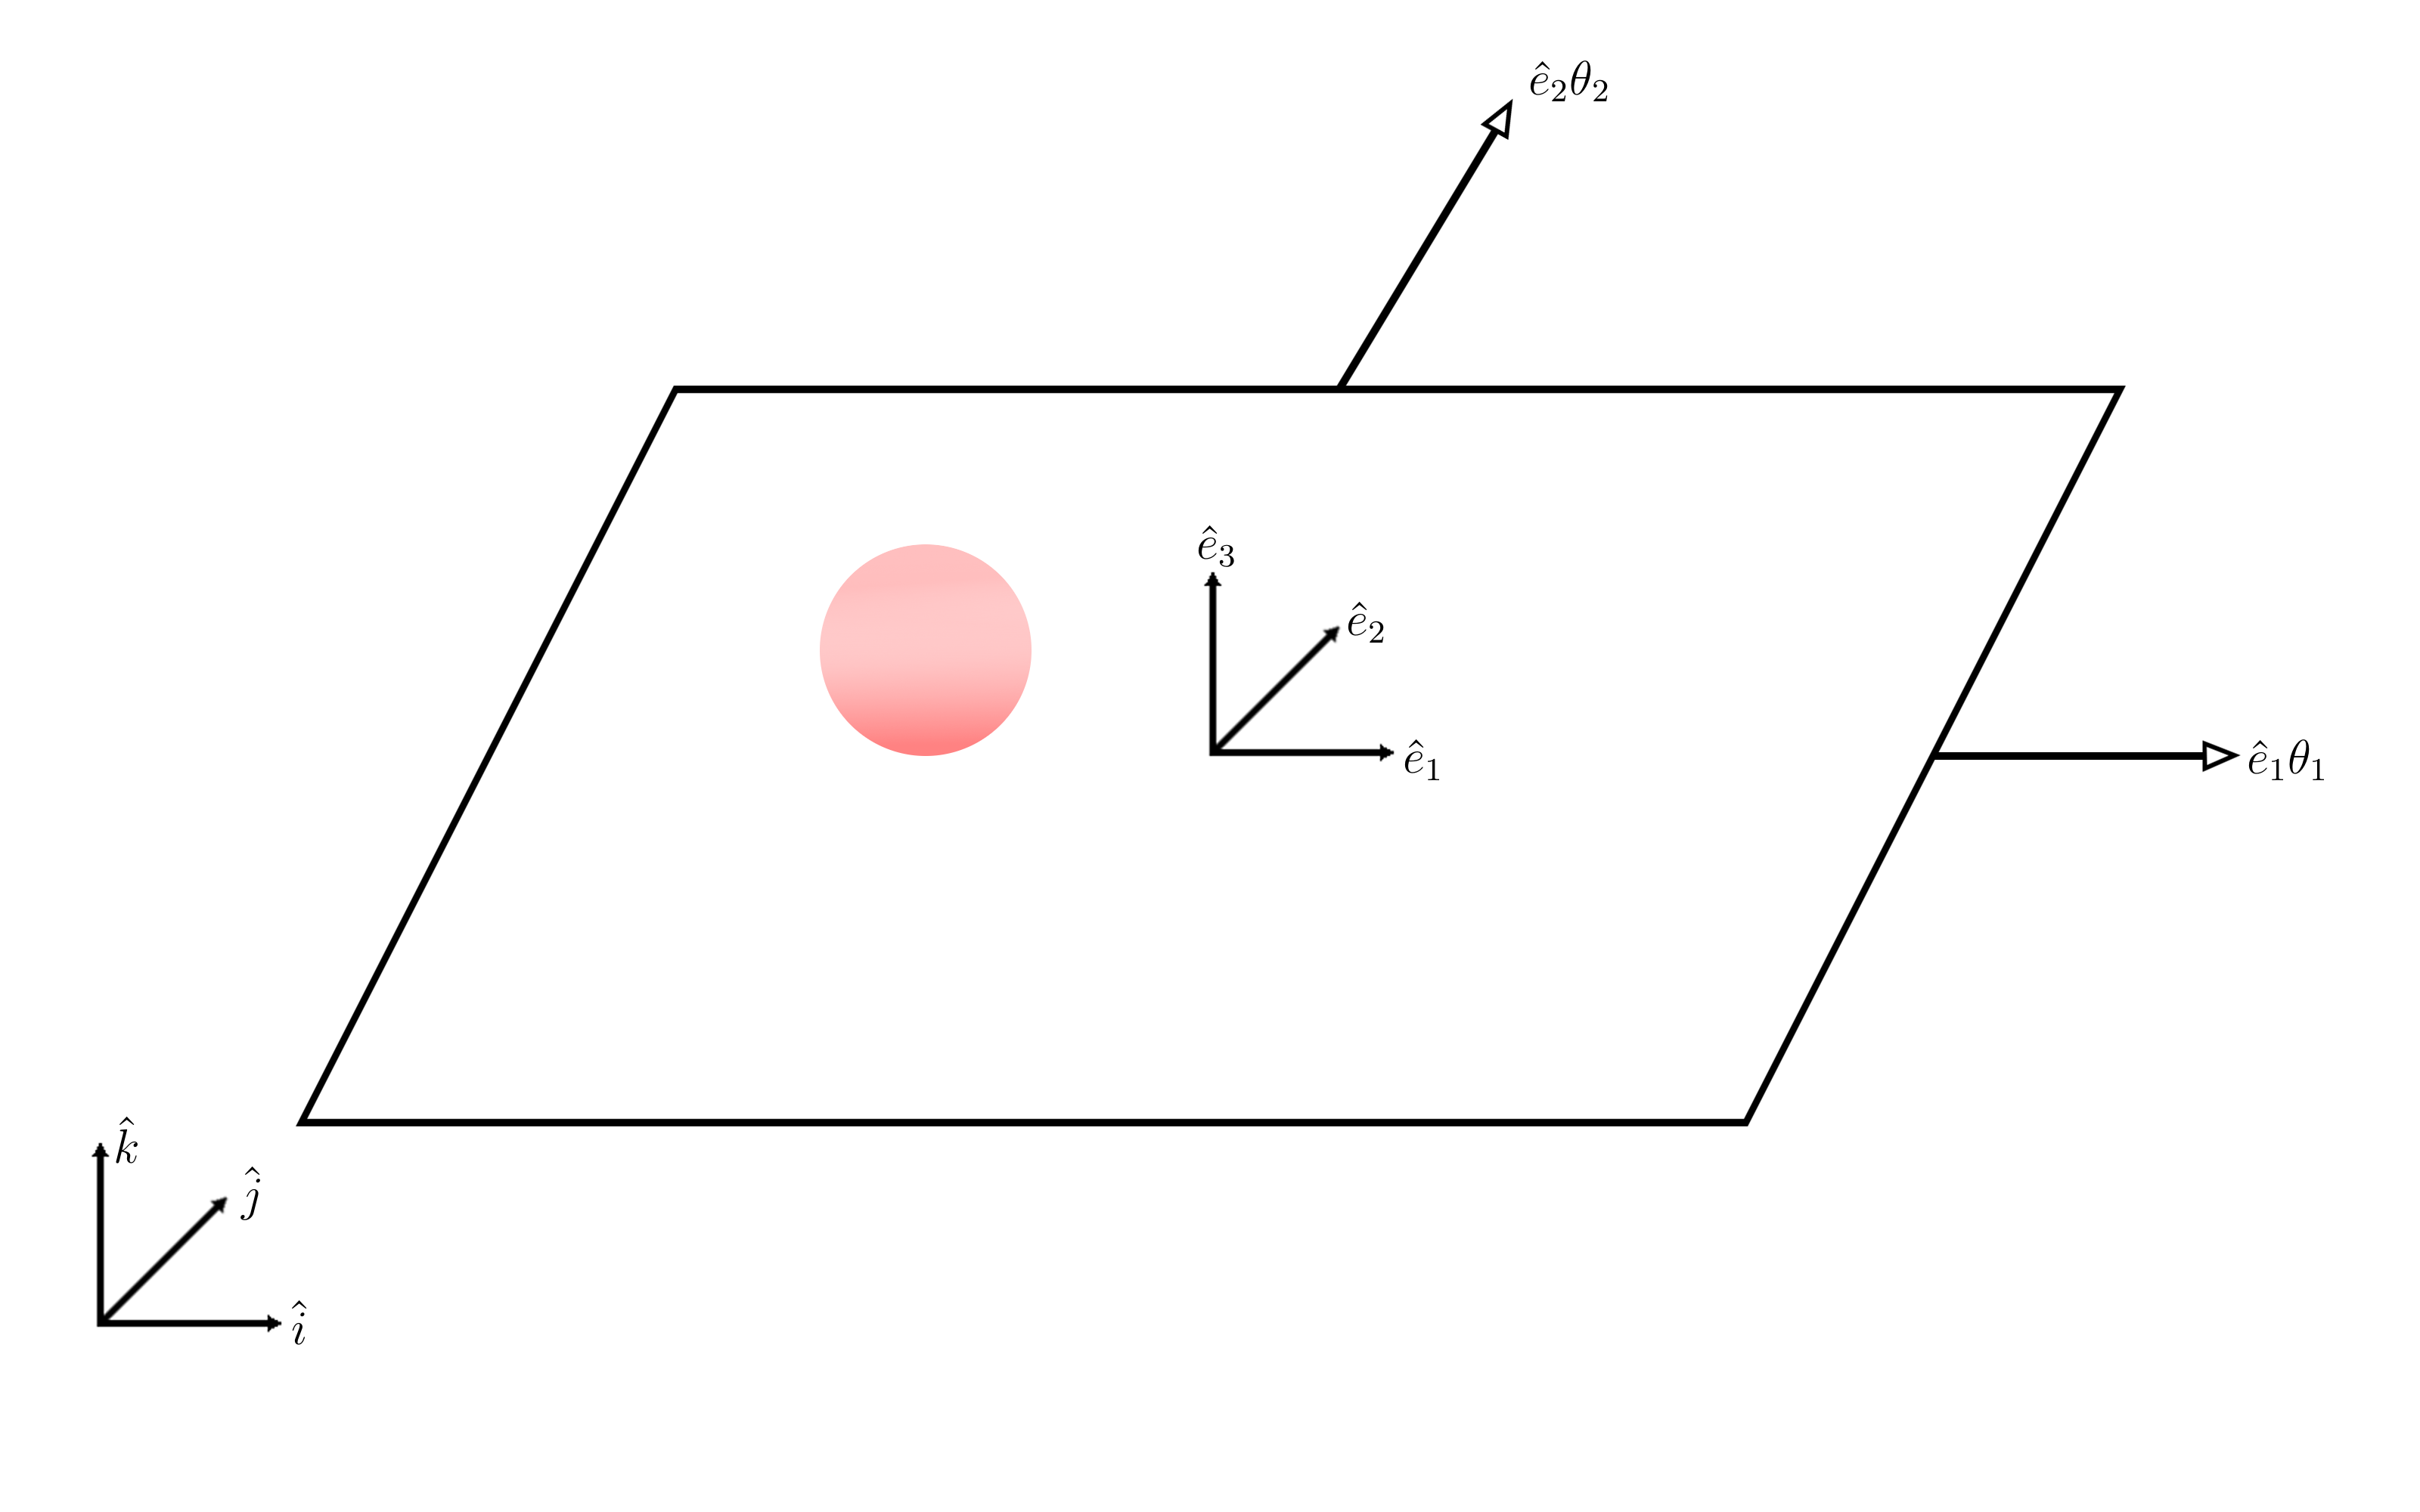
\includegraphics[width=\textwidth]{bap2}
	\caption{Ball and Plate, modello fisico}
	\label{figure:bap}
\end{figure}

\subsection{Cinematica Ball and Plate}

In figura \ref{figure:bap} vengono mostrati i sistemi di riferimento solidali allo spazio $\{\hat{i}, \hat{j}, \hat{k}\}$ e solidali al piano $\{\hat{e}_{1}, \hat{e}_{2}, \hat{e}_{3}\}$. Con gli angoli $\theta_{1} = \theta_{2} = 0$ i due sistemi di riferimento sono equivalenti.

La matrice di rotazione ottenuta nell'ordine di rotazione di $\theta_{2}\hat{e}_{2}$ seguita da $\theta_{1}\hat{e}_{1}$ è la seguente:

\begin{equation}
	\begin{pmatrix}
		\hat{e}_{1} \\
		\hat{e}_{2} \\
		\hat{e}_{3}
	\end{pmatrix}=
	\begin{pmatrix}
		\cos\theta_{2}		&&		\sin\theta_{1}\cos\theta_{2}		&&		-\cos\theta_{1}\sin\theta_{2}		\\
		0					&&		\cos\theta_{1}						&&		\sin\theta_{1}						\\
		\sin\theta_{2}		&&		-\sin\theta_{1}\cos\theta_{2}		&&		\cos\theta_{1}\cos\theta_{2}
	\end{pmatrix}
	\begin{pmatrix}
		\hat{i}		\\
		\hat{j}		\\
		\hat{k}
	\end{pmatrix}
\end{equation}
\newpage
La matrice inversa permette di ottenere il cambio di coordinate nell'equazione \ref{equation:bap1}:

\begin{equation}
	\begin{pmatrix}
		\hat{i}	\\
		\hat{j} \\
		\hat{k}
	\end{pmatrix}=
	\Theta
	\begin{pmatrix}
		\hat{e}_{1} \\
		\hat{e}_{2} \\
		\hat{e}_{3}
	\end{pmatrix}
	\label{equation:bap1}
\end{equation}

In cui $\Theta$ assume il valore presente nell'equazione \ref{equation:theta}:

\begin{equation}
	\Theta=
	\begin{pmatrix}
		\cos\theta_{2}					&&		0					&&		\sin\theta_{2}					\\
		\sin\theta_{1}\sin\theta_{2}	&&		\cos\theta_{1}		&&		-\cos\theta_{2}\sin\theta_{1}	\\
		-\cos\theta_{1}\sin\theta_{2}	&&		\sin\theta_{1}		&&		\cos\theta_{1}\cos\theta_{2}
	\end{pmatrix}
	\label{equation:theta}
\end{equation}

Indicando con $\rho$ la posizione della sfera sul piano in termini di coordinate legate al piano, otteniamo la posizione della sfera nel sistema di riferimento dello spazio:

\begin{equation}
	\begin{pmatrix}
		\hat{i}	\\
		\hat{j} \\
		\hat{k}
	\end{pmatrix}=
		\Theta\rho=
		\Theta
		\begin{pmatrix}
			x_{p}\\
			y_{p}\\
			r
		\end{pmatrix}
	\label{equation:rho}
\end{equation}

In cui $x_{p}$ e $y_{p}$ sono la posizione della sfera nel piano, e $r$ è il raggio della sfera.


\subsection{Dinamica Ball and Plate}

Le equazioni differenziali del moto del sistema Ball and Plate sono visualizzabili nelle equazioni \ref{equation:motobapx} e \ref{equation:motobapy}:

\begin{equation}
	\begin{split}
		\ddot{x}_{p}=\frac{5}{7}[g\cos\theta_{1}\sin\theta_{2}+\sin\theta_{2}(-r\cos\theta_{2}+x_{p}\sin\theta_{2})\dot{\theta}_{1}^2	\\
			+x_{p}\dot{\theta}_{2}+2\sin\theta_{2}\dot{\theta}_{1}\dot{y}_{p}+y_{p}\sin\theta_{2}\ddot{\theta}_{1}]-r\ddot{\theta}_{2}
	\end{split}
	\label{equation:motobapx}
\end{equation}
\begin{equation}
	\begin{split}
		\ddot{y}_{p}=\frac{5}{7}[-g\sin\theta_{1}+y_{p}\dot{\theta}_{2}^2-\frac{12}{5}r\sin\theta_{2}\dot{\theta}_{1}\dot{\theta}_{2}-2\sin\theta_{2}\dot{\theta}_{1}\dot{x}_{p}	\\
		-x_{p}(2\cos\theta_{2}\dot{\theta}_{1}\dot{\theta}_{2}+\sin\theta_{2}\ddot{\theta}_{1})+r\cos\theta_{2}\ddot{\theta}_{1}
	\end{split}
	\label{equation:motobapy}
\end{equation}

La sfera di raggio r è posta sul piano inclinabile attorno ad un giunto tramite l'uso di un servomotore. Dato che il giunto è vincolato al piano mediante una staffa di altezza $h$, il centro di massa del sistema è traslato. È quindi necessario modificare le equazioni \ref{equation:motobapx} e \ref{equation:motobapy} come segue:

\begin{equation}
\begin{split}
\ddot{x}_{p}=\frac{5}{7}[g\cos\theta_{1}\sin\theta_{2}+\sin\theta_{2}(-(r+h)\cos\theta_{2}+x_{p}\sin\theta_{2})\dot{\theta}_{1}^2	\\
+x_{p}\dot{\theta}_{2}+2\sin\theta_{2}\dot{\theta}_{1}\dot{y}_{p}+y_{p}\sin\theta_{2}\ddot{\theta}_{1}]-(r+\frac{5}{7}h)\ddot{\theta}_{2}
\end{split}
\label{equation:motobapxmod}
\end{equation}
\begin{equation}
\begin{split}
\ddot{y}_{p}=\frac{5}{7}[-g\sin\theta_{1}+y_{p}\dot{\theta}_{2}^2-2(\frac{6}{5}r+h)\sin\theta_{2}\dot{\theta}_{1}\dot{\theta}_{2}-2\sin\theta_{2}\dot{\theta}_{1}\dot{x}_{p}	\\
-x_{p}(2\cos\theta_{2}\dot{\theta}_{1}\dot{\theta}_{2}+\sin\theta_{2}\ddot{\theta}_{1})+(r+\frac{5}{7}h)\cos\theta_{2}\ddot{\theta}_{1}
\end{split}
\label{equation:motobapymod}
\end{equation}

Inoltre, è possibile osservare la relazione tra l'angolo d'inclinazione del piano e quello del servomotore:

\begin{equation}
\theta_{2}=\sin^{-1}(\frac{d}{l_{x}}\sin\alpha)
\label{equation:approximation}
\end{equation} 

Dove $d$ è la lunghezza del braccio del motore vincolato al suo asse di rotazione, $l_{x}$ è la lunghezza del piano x e $\alpha$ è l'angolo del servomotore rispetto alla direzione $\hat{i}$,

\subsection{Semplificazione del modello}

Al fine di semplificare il modello è possibile osservare che per $\theta_{1}=\theta_{2}=0$ ci sono infiniti punti di equilibrio $x_{p},y_{p}$. Supponendo che ci siano piccole variazioni di angoli nell'intorno di questo punto è possibile affermare che $\sin\theta\approx\theta$ e $\cos\theta\approx1$. Inoltre i piccoli cambiamenti di inclinazione del piatto nell'intorno del punto di equilibrio possono sempre essere tradotti con:
\begin{align}
	\centering
	\ddot{\theta}_{1}=\dot{\theta}_{1}=\theta_{1}=\dot{y}_{p} &\cong0 \\
	\ddot{\theta}_{2}=\dot{\theta}_{2}=\theta_{2}=\dot{x}_{p} &\cong0
\end{align}

Rispettivamente nelle equazioni di $\ddot{x}_{p}$ e $\ddot{y}_{p}$. Le equazioni del moto \ref{equation:motobapxmod} e \ref{equation:motobapymod} possono quindi essere nuovamente riscritte:

\begin{align}
	\ddot{x}_{p} &= \frac{5}{7}g\theta_{2}-(r+\frac{5}{7}h)\ddot{\theta}_{2}	\label{align:1}	\\
	\ddot{y}_{p} &= -\frac{5}{7}g\theta_{1}+(r+\frac{5}{7}h)\ddot{\theta_{1}}	\label{align:2}
\end{align}

Approssimando anche la relazione \ref{equation:approximation} si ha che:

\begin{align}
	\theta_{2} &= \frac{d}{l_{x}}\alpha	\\
	\theta_{1} &= \frac{d}{l_{y}}\beta
\end{align}

In cui $l_{x}$ e $l_{y}$ sono le lunghezze del piano rispettivamente lungo x e lungo y, e $\alpha$ e $\beta$ sono gli angoli impostati dai servomotori. È anche possibile trascurare l'ultimo termine delle equazioni \ref{align:1} e \ref{align:2}, che rappresenta la forza centrifuga dovuta alla rotazione del piano. Le equazioni finali sono quindi:

\begin{align}
	\ddot{x}_{p} &= \frac{5}{7}g\frac{d}{l_{x}}\alpha	\label{equation:bapfinalx}	\\
	\ddot{y}_{p} &= -\frac{5}{7}g\frac{d}{l_{y}}\beta	\label{equation:bapfinaly}
\end{align}

\subsection{Modello nello spazio di stato}

Possiamo definire un vettore $x$ di stato e un vettore $u$ di ingresso al sistema come segue:
\begin{equation}
	x=
	\begin{bmatrix}
		x_{p}		\\
		\dot{x}_{p}	\\
		y_{p}		\\
		\dot{y}_{p}
	\end{bmatrix}
	;
	u=
	\begin{bmatrix}
		\alpha	\\
		\beta
	\end{bmatrix}
\end{equation}

Con uscita diretta dello stato

\begin{align}
	\begin{cases}
		\dot{x}(t) &= Ax(t) + Bu(t)	\\
		y(t) &= Cx(t)
	\end{cases}
\end{align}

Definendo le matrici dello spazio di stato come:

\begin{equation}
	A=
	\begin{bmatrix}
		0 && 1 && 0 && 0 \\
		0 && 0 && 0 && 0 \\
		0 && 0 && 0 && 1 \\
		0 && 0 && 0 && 0
	\end{bmatrix}
	;
	B=
	\begin{bmatrix}
		0	&&	0	\\
		\dfrac{5}{7}g\dfrac{d}{l_{x}}	&&	0	\\
		0	&&	0	\\
		0	&& -\dfrac{5}{7}g\dfrac{d}{l_{y}}
	\end{bmatrix}
	;
	C=
	\begin{bmatrix}
	1 && 0 && 0 && 0 \\
	0 && 0 && 1 && 0
	\end{bmatrix}
\end{equation}

Lo spazio di stato è composto da due sottosistemi indipendenti tra loro, per cui è possibile dividerlo in due sistemi, uno che riproduce le dinamiche lungo l'asse $x$ e l'altro che rappresenta le dinamiche lungo l'asse $y$:

\begin{align}
	Dinamica\ asse\ x:
	\begin{cases}
		\dot{x}_{1}&=
		\begin{bmatrix}
			\dot{x}_{p} \\ \ddot{x}_{p}
		\end{bmatrix}
		=
		\begin{bmatrix}
			0 && 1 \\ 0 && 0
		\end{bmatrix}
		\begin{bmatrix}
			x_{p}	\\ \dot{x}_{p}
		\end{bmatrix}
		+
		\begin{bmatrix}
			0	\\	\dfrac{5}{7}g\dfrac{d}{l_{x}}
		\end{bmatrix}
		\alpha
		\\
		y_{1}&=
		\begin{bmatrix}
			1 && 0
		\end{bmatrix}
		\begin{bmatrix}
			x_{p} \\ \dot{x}_{p}
		\end{bmatrix}
	\end{cases}
\end{align}

\begin{align}
	Dinamica\ asse\ y:
	\begin{cases}
		\dot{x}_{2}&=
		\begin{bmatrix}
			\dot{y}_{p} \\ \ddot{y}_{p}
		\end{bmatrix}
		=
		\begin{bmatrix}
			0 && 1 \\ 0 && 0
		\end{bmatrix}
		\begin{bmatrix}
			y_{p}	\\ \dot{y}_{p}
		\end{bmatrix}
		+
		\begin{bmatrix}
			0	\\	-\dfrac{5}{7}g\dfrac{d}{l_{y}}
		\end{bmatrix}
		\beta
		\\
		y_{2}&=
		\begin{bmatrix}
			1 && 0
		\end{bmatrix}
		\begin{bmatrix}
			y_{p} \\ \dot{y}_{p}
		\end{bmatrix}
	\end{cases}
\end{align}

\newpage
\subsection{Componenti utilizzati}

In questa sottosezione sono elencati i vari componenti utilizzati.

\begin{itemize}[noitemsep]
	\item Arduino Mega 2560
	\item Touch screen resistivo a 4 pin
	\item 2 servomotori Hitec HS 300
	\item Plancia ball and plate Evidence Amazing Ball\cite{plancia}
\end{itemize}

\subsection{Riparazione della Ball and Plate}

\subsubsection{Riparazione del touch screen resistivo}

Al momento dell'inizio dei lavori, il gruppo si è accorto che il touch screen resistivo presentava della anomalie nella misura: infatti, l'area coperta dal sensore non era di forma rettangolare come previsto, ma aveva una forma trapezioidale molto irregolare. Il team ha perciò iniziato a calcolare dei modi per "mappare" le coordinate fallate del trapezio irregolare per farle combaciare con quelle di un rettangolo. Ciononostante, durante una delle prove la sfera è scivolata colpendo con forza il touchscreen, che ha ripreso di seguito a funzionare normalmente. La nostra ipotesi è che, a causa dell'inutilizzo e magari di alcuni agenti esterni, le due sezioni del touch screen erano rimaste praticamente "incollate" causando così l'anomalia nella misura, e che il forte colpo ricevuto abbia (fortunatamente) interrotto questo contatto perenne permettendo al sensore di riprendere il suo normale funzionamento.

\subsubsection{Sostituzione di un servomotore}

Uno dei due servomotori montati sul sistema aveva un funzionamento lento e oscillante. Dopo varie sedute di prova si è bruciato, per cui il team ha dovuto sostituirlo con un altro dello stesso tipo. Ciononostante, il sistema presenta comunque un comportamento oscillatorio, cosa che il gruppo attribuisce alla scarsa qualità dei motori che, purtroppo, è stato impossibile sostituire con modelli più recenti ed adatti allo scopo.

\subsection{Misure della Ball and Plate}

In tabella \ref{table:misure} sono riportate le misure fisiche del sistema Ball and Plate preso in considerazione:

\begin{table}[ht]
	\centering
	\begin{tabular}{|c|c|}
		\hline
		\rowcolor[HTML]{C0C0C0} 
		Parametro 		& Valore   \\ \hline
		$h$         	& 0.036    \\ \hline
		$r$         	& 0.0135   \\ \hline
		$d$         	& 0.015    \\ \hline
		$l_{x}$     	& 0.23     \\ \hline
		$l_{y}$     	& 0.18     \\ \hline
	\end{tabular}
	\caption{Misure fisiche del sistema Ball and Plate}
	\label{table:misure}
\end{table}

